\documentclass[../TDE1-E2.tex]{subfiles}%

\begin{document}
\section[s]"1"{Résistances équivalentes}
\QR{%
  Exprimer la résistance équivalente à l'association de deux résistances
          $R_1$ et $R_2$ placées en parallèle.
}{%
  \vspace{-15pt}
  \begin{tcbraster}[raster columns=2, raster equal height=rows]
    \begin{tcn}(ques){Résultat attendu}
      \begin{center}
        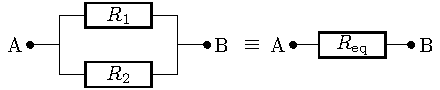
\includegraphics{2parrequiv}
      \end{center}
    \end{tcn}
    \begin{tcn}(tool)'r'{Outil}
      L'association en parallèle de deux résistances $R_1$ et $R_2$ donne une
      résistance équivalente $ R_{\rm eq}$ telle que~:
      \begin{empheq}[box=\fbox]{equation*}
        \frac{1}{ R_{\rm eq}} = \frac{1}{R_1} + \frac{1}{R_2}
      \end{empheq}
    \end{tcn}
    \begin{tcn}(impo){Attention !}
      Faites particulièrement attention à bien écrire $\DS \frac{1}{
      R_{\rm eq}}$ et non pas simplement $ R_{\rm eq}$, même après 5
      lignes de calcul quand c'est nécessaire. Pensez toujours à
      vérifier l'homogénéité d'un résultat littéral avant de l'encadrer.
      Cette erreur est une des plus communes.
    \end{tcn}
    \begin{tcn}(appl)'r'{Application}
      En mettant les deux termes sur même dénominateur~:
      \begin{align*}
        \frac{1}{ R_{\rm eq}}                 & = \frac{1}{R_1}\times \textcolor{orange}{
          \frac{R_2}{R_2}} + \frac{1}{R_2}\times \textcolor{orange}{
        \frac{R_1}{R_1}}                                                                  \\
        \Leftrightarrow \frac{1}{ R_{\rm eq}} & = \frac{R_2 + R_1}{R_1R_2}                \\
        \Leftrightarrow R_{\rm eq}            & = \frac{R_1R_2}{R_1+R_2}
      \end{align*}
    \end{tcn}
  \end{tcbraster}
}%

\QR{%
  Que devient cette expression si $R_1 = R_2$~?
}{%
  ~
  \vspace{-15pt}
  \begin{center}
    \begin{tcn}[width=\linewidth](appl){Application}
      \[R_1 = R_2 = R \Longrightarrow \boxed{ R_{\rm eq} = \frac{R}{2}}\]
    \end{tcn}
  \end{center}
}%

\QR{%
  Exprimer la résistance équivalente à l'association des résistances
          $R_1$, $R_2$ et $R_3$ placées en parallèle.
}{%
  \vspace{-15pt}
  \begin{tcbraster}[raster columns=2, raster equal height=rows]
    \begin{tcn}(ques){Résultat attendu}
      \begin{center}
        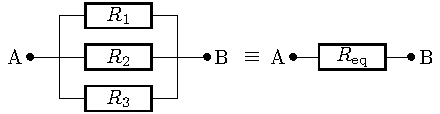
\includegraphics{3parrequiv}
      \end{center}
    \end{tcn}
    \begin{tcn}(tool)'r'{Outil}
      L'association en parallèle de trois résistances $R_1$, $R_2$ et
      $R_3$ donne une résistance équivalente $ R_{\rm eq}$ telle que~:
      \begin{empheq}[box=\fbox]{equation*}
        \frac{1}{ R_{\rm eq}} = \frac{1}{R_1} + \frac{1}{R_2} + \frac{1}{R_3}
      \end{empheq}
    \end{tcn}
  \end{tcbraster}
  \begin{center}
    \begin{tcn}[width=\linewidth](appl){Application}
      De la même manière que précédemment, la mise sous même dénominateur
      donne~:
      \begin{gather*}
        \frac{1}{ R_{\rm eq}}       = \frac{R_2R_3}{R_1R_2R_3} +
        \frac{R_1R_3}{R_1R_2R_3} + \frac{R_1R_2}{R_1R_2R_3}
        \Lra
        R_{\rm eq}  = \frac{R_1R_2R_3}{R_1R_2 + R_2R_3 +
          R_1R_3}
      \end{gather*}
      qui est bien homogène à une résistance étant de la forme $\DS
        \frac{R^{\cancel{3}}}{\cancel{R^2}} = R$.
    \end{tcn}
  \end{center}
}%

\QR{%
  Que devient cette expression si $R_1 = R_2 = R_3$~?
}{%
  ~
  \vspace{-15pt}
    \begin{tcn}[width=\linewidth](appl){Application}
      \[R_1 = R_2 = R_3 = R \Longrightarrow R_{\rm eq} = \frac{R^3}{3R^2}
        \Leftrightarrow \boxed{R_{\rm eq} = \frac{R}{3}}\]
    \end{tcn}
}%

\QR{%
  Exprimer la résistance équivalente à l'association de $n$ résistances
          identiques placées en parallèle.
}{%
  \vspace{-15pt}
  \begin{tcbraster}[raster columns=2, raster equal height=rows]
    \begin{tcn}(ques){Résultat attendu}
      \begin{center}
        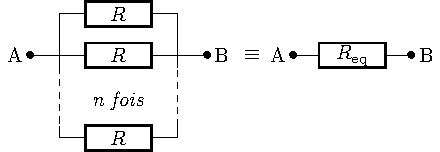
\includegraphics{nparrequiv}
      \end{center}
    \end{tcn}
    \begin{tcn}(appl)'r'{Application}
      Il n'y a toujours qu'une seule formule attendue, et elle s'écrit~:
      \[ \frac{1}{R_{\rm eq}} = \underbrace{ \frac{1}{R} + \frac{1}{R} +
          \cdots + \frac{1}{R}}_{\textit{n fois}} \Leftrightarrow
        \boxed{R_{\rm eq} = \frac{R}{n}} \]
    \end{tcn}
  \end{tcbraster}
}%

\end{document}
